%----------------------------------------------------------------------------
\chapter{\bevezetes}
%----------------------------------------------------------------------------

Subgraph isomorphism is an NP-hard problem which has many application areas.
It is called substructure search in cheminformatics and it is used to find
similar molecular compounds based on their structural formula. In bioinformatics,
complex biological systems are decomposed into several different networks,
such as protein-protein interaction, metabolic interaction or hormone signaling
networks, which are represented as graphs. Analyzing and understanding these
large networks requires finding certain topological patterns, i.e. subgraph
isomorphism. 

Graph pattern matching is also a core concept of social network analysis.
Such graphs tend to be extremely large with millions of vertices and billions
of edges in the real world. Although subgraph isomorphism has been extensively
studied in the past, there was a renewed interest in the topic recently, which
yielded some notable results. The newer algorithms significantly out-perform
the previous state-of-the-art solutions (Ullman's algorithm \cite{Ullmann1976AnAF} \cite{ullmanimpr}, VF2 \cite{vf2} ), sometimes even 
in order of magnitudes. This made it possible to query subgraph isomorphisms
in such large graphs. However social networks are not static. In practice, they
are frequently updated with typically small changes like adding or removing edges.
Despite the changes being small, they will still have an impact on the matches.
This means that the matches have to be re-computed from scratch on every update,
which is highly infeasible even with the newer and faster subgraph isomorphism
algorithms. To minimize unnecessary re-computations, incremental algorithms
can be used, that compute the changes in matches based on the changes in the
search graph.

\cite{incrementalpatternmatching} discusses in depth several types of incremental graph pattern matching algorithms.
However the authors' topic of interest in \cite{incrementalpatternmatching2} and \cite{incrementalpatternmatching} is incremental graph pattern matching
with (bounded) graph simulation. A graph \(G\) matches a pattern \(q\) via graph 
simulation if there exists a binary relation \(S \subseteq V_q \times V\) such that 
\begin{enumerate}
    \item for each \(u \in V_q\), there exists \(v \in V\) such that \((u, v) \in S\);
    \item for each \((u, v) \in S\), 
        \begin{enumerate}
            \item \(\mathcal{L}(u) = \mathcal{L}(v)\), and
            \item for each edge \((u, u') \in E_q\), there exists a non-empty path \(\rho = v \rightsquigarrow v'\) in \(G\) such that \((u', v') \in S\) and the length of \(\rho\) is less than the maximum allowed length defined on the given edge in \(q\).
        \end{enumerate}
\end{enumerate}
Graph simulation is less strict about the topology of its results than graph
isomorphism. This can be beneficial if we want to express loose connections in
our query patterns, and on top of that, pattern matching with graph simulation
can be done in \(\mathcal{O}(n^3)\). However if we do require strict matches,
only subgraph isomorphism can come into play. Although the authors provided an
incremental algorithm for subgraph isomorphism, it was more of a demonstration
that even in an NP-hard case, computing matches incrementally (which is also
NP-hard) can out-perform a fast solution, VF2. The approach introduced there
does not take full advantage on previous computations, and it was also not 
evaluated in much detail. Note that this was not the main focus of the paper.

In this work, we investigate how two state-of-the-art algorithms (VF2++, DAF)
can be converted into their incremental version. First, we give an introduction
how the two algorithms work. Then we describe a method to make them incremental.
Finally, we evaluate the results both in terms of complexity and practical
measurements.

\section{Background}

\begin{definition}[Graph]
    A graph is a pair \(G = (V,E)\), where \(V\) is a set of vertices,
    \(E\) is a set of paired vertices that denotes the undirected edges 
    of the graph. 
\end{definition}

\begin{definition}[Labelling]
    \( \mathcal{L} : V \rightarrow K \), is a vertex labelling function 
    which maps vertices into arbitrary sets whose elements are the labels
    of the given node. Two vertices, \(u, v\) are equivalent if 
    \( \mathcal{L}(u) = \mathcal{L}(v) \).
\end{definition}

\begin{definition}[Isomorphism]
    \(G_1\) and \(G_2\) are isomorphic if a bijection exists between \(V_1\)
    and \(V_2\) such that two vertices are neighbours in \(G_1\) if and only
    if their respective pairs in \(G_2\) are neighbours, neighbouring 
    vertex pairs have the same number of edges between each other, and a
    vertex and its pair have the same labels.
\end{definition}

\begin{definition}[Subgraph]
    \(G_1\) is a subgraph of \(G_2\) if \(V_1 \subseteq V_2 \), \(E_1 \subseteq E_2\)
    and two vertices are neighbours in \(G_1\) only if they are neighbours in \(G_2\).
\end{definition}

\begin{definition}[Induced subgraph]
    If \(E_1\) consists of those edges from \(E_2\) whose both vertices are in
    \(V_1\), and \(E_1\) contains all these edges, then \(G_1\) is an induced
    subgraph of \(G_2\).
\end{definition}

\begin{definition}[Subgraph isomorphism]
    \(G_1\) is subgraph isomorphic to \(G_2\) if \(G_1\) is isomorphic to any
    subgraphs of \(G_2\).
\end{definition}

\begin{definition}[Induced subgraph isomorphism]
    \(G_1\) is induced subgraph isomorphic to \(G_2\) if \(G_1\) is isomorphic to any
    induced subgraphs of \(G_2\). Throughout this paper, we refer to induced subgraph
    isomorphism with the term of subgraph isomorphism. $M(q, G)$ denotes the set of 
    mappings found by an arbitrary subgraph isomorphism algorithm.
\end{definition}

\begin{definition}
    An injection $m : D \rightarrow V_G$ is called a (partial) mapping, where $D \subseteq V_q$.
\end{definition}

\begin{definition}
    $m_q$ and $m_G$ denotes the domain and the range of m respectively.
\end{definition}

\begin{definition}
    A mapping $m$ covers a node $u \in V_q \cup V_G$ if $u \in m_q \cup m_G$.
\end{definition}

\begin{definition}
    A mapping $m$ is a whole mapping if it covers all the nodes of $V_q$.
\end{definition}


This paper concentrates on the induced subgraph isomorphism problem in dynamic graphs, 
i.e. graphs that change with time. After finding the initial matches given a query graph
\(q\) and a data graph \(G\), keep the set of matches up to date in response to small 
updates \(\Delta G \) on \(G\) without recomputing all matches from scratch. \(\Delta G\) 
can be one of the following operations:
\begin{itemize}
    \item add a new node to \(G\),
    \item remove an existing node from \(G\),
    \item add an edge between two nodes of \(G\) and
    \item remove an existing edge between two nodes of \(G\).
\end{itemize}

\section{Algorithms}

This section gives a brief overview on how the two algorithms of interest (DAF and VF2++)
work.

\subsection{VF2}

Since VF2++ is an extension over VF2, first, we describe how VF2 works. It is a recursive 
algorithm where each state of the matching process can be associated with a partial mapping
$m$. VF2 starts with an empty mapping and it 
gradually extends it until a whole mapping is reached. For the current mapping $m$, it calculates a 
candidate set of $(u, v)$ pairs to be included in $m$. It iterates over the
$(u, v)$ elements of the candidate set, and if $\mathcal{F}(m, (u, v))$ is feasible then it recursively 
tries to extend $m'$, where $\mathcal{F}$ is the feasibility function and $m'$ is a partial mapping
obtained by adding $(u, v)$ to $m$.

\begin{definition}
    Let $m$ be a mapping. $Cons(m, (u, v))$ is a logical consistency function which is true if and only if $m$
    satisfies the requirements of induced subgraph isomorphism considering $q_m$ and $G_m$, where
    $q_m$ and $G_m$ are the subgraphs of $q$ and $G$ induced by $m_q$ and $m_G$
    respectively. $Cons$ is used to verify that the consistency of $m$ also holds after extended with $(u, v)$.
\end{definition}

\begin{definition}
    Let $m$ be a mapping. $Cut(m)$ is a logical cutting function which is false if there exists a 
    sequence of extensions of $m$ for which the resulting mapping is whole and it satisfies the
    requirements of induced subgraph isomorphism. $Cut$ is used to determine if the current partial 
    mapping is not contained in any whole mapping, thus trying to extend it would be useless.
\end{definition}

\begin{definition}
    The feasibility function $\mathcal{F}$ is defined as follows: 
    
    $\mathcal{F}(m, (u, v)) = Cons(m, (u, v)) \land \neg Cut(m)$.
\end{definition}

The feasibility function ensures that the algorithm considers only $(u, v)$ candidates such that 
$m$ extended with $(u, v)$ remains consistent, and it eliminates the need of processing partial
mappings for which it can be proven that they cannot be extended to a whole mapping.

\begin{algorithm}[h]
    \SetAlgoLined\DontPrintSemicolon
    \SetKwFunction{proc}{vf2}
    \SetKwProg{myproc}{Procedure}{}{}
    \myproc{\proc{m}}{
        \uIf(){$m$ covers $V_q$}{
            \nl Output(m)\;
        }
        \Else{
            \nl $P_m$ $\gets$ the candidate set of pairs for extending $m$\;
            \ForEach(){$(u, v) \in P_m$}{
                \uIf(){$\mathcal{F}(m, (u, v))$}{
                    \nl \proc(extend($m, (u,v)$))\;
                }
            }
        }        
    }
    \caption{VF2 algorithm}
\end{algorithm}

Let $T_q(m) := {u \in V_q \ m_q: \exists u' \in m_q: (u, u') \in E_q}$, and
$T_G(m) := {v \in V_G \ m_G: \exists v' \in m_G: (v, v') \in E_G}$.

The candidate set for extending $m$ is $P_m$. $P_m$ consists of the pairs of uncovered neighbors
of covered nodes. If there exists no such pair, $P_m$ contains all uncovered nodes. Formally,

\[
    P_m = 
\begin{cases}
    T_q(m) \times T_G(m),& \text{if} T_q(m) \neq \emptyset \text{and} T_G(m) \neq \emptyset\\
    (V_q \setminus m_q) \times (V_G \setminus m_G),  & \text{otherwise}.
\end{cases}    
\]


\subsection{VF2++}

VF2++ \cite{vf2pp} was published by Alp\'{a}r J\"{u}ttner and P\'{e}ter Madarasi in 2018.
The algorithm makes performance improvements compared to VF2 by calculating a matching
order, in which the vertices of $q$ are processed in a partial mapping, and by applying
a more efficient cutting function.

The order of the nodes of $q$ to be matched have a huge impact on the number of visited
states. In case of VF2, the lack of strictly defined matching order can lead to evaluating
states that cannot be wholly extended, only to realize this deep down on the search tree.
By choosing a proper matching order, one can eliminate such unnecessary computations earlier.

\begin{example}
    The following example was taken from the original VF2++ paper. Let $q$ be a query graph 
    that cannot be mapped to $G$, and $u \in V_q$. Let 
    $q' := V_q \cup \{u'_1, u'_2,\cdots,u'_k\}, E_q \cup \{ (u, u'_1),(u'_1, u'_2),\cdots,(u'_{k-1}, u'_k) \}$,
    i.e. $q'$ is the same graph as $q$ which was extended with a $k$ long path, which is disjoint
    from $q$ and one of its starting nodes is connected to $u \in V_q$.

    If the first $k$ vertices in the matching order were the nodes of the newly added path,
    VF2 would iterate through all possible $k$ long paths in $G$, only to realize that no
    partial mappings can be extended to $q'$.

    However, if it started the matching process with vertices from $q$, it would not have
    matched any nodes from the path.
\end{example}


The first step of VF2++ is determining the matching order in which the algorithm will process
the vertices of the query graph $q$. During the order's computation, VF2++ takes into account
the structure of $q$ and its labeling. First, it chooses a node with the least common label 
and with the largest degree. This node will be the root of a tree, which will be used to determine
the final matching order $\mathcal{O}$.


\[ root = {r | r \in \argmax_{deg}(\argmin_{label_{\mathcal{O}}}(V_q \setminus \mathcal{O}))} \]
, where $label_{\mathcal{O}}(n) := |{v \in V_G : \mathcal{L}(n) = \mathcal{L}(v)}| - |{u \in \mathcal{O}: \mathcal{L}(n) = \mathcal{L}(u)}|$, 
i.e. it computes the difference between the number of vertices in $G$ with the label of $n$ and 
the number of vertices in $\mathcal{O}$ with the label of $n$. Next, the algorithm computes a tree 
$T$ by traversing $q$ in BFS (Breadth first search) order from the previously calculated root, and
it processes each level of $T$ the following way. Let $V_{q,d}$ denote the set of vertices of $T$ in
depth $d$. The process selects the vertices with the largest connectivity respect to $\mathcal{O}$,
i.e. those nodes whose number of neighbors that are already in $\mathcal{O}$ is the largest. Then
from these nodes, it selects the ones with the largest degree, then those with the rarest label.

\[ o = {u | u \in \argmin_{label_{\mathcal{O}}}(\argmax_{deg}(\argmax_{conn}(V_{q,d})))} \]

The selected node $o$ is appended to $\mathcal{O}$, and it is removed from $V_{q,d}$. This continues 
until $V_{q,d}$ has no more elements. Algorithm \ref{alg:vf2pporder} and \ref{alg:vf2ppproc} describe
the matching order procedures on a high level.

\begin{algorithm}[h]
    \SetAlgoLined\DontPrintSemicolon
    \SetKwFunction{proc}{vf2\_order}
    \SetKwFunction{process}{process}
    \SetKwProg{myproc}{Procedure}{}{}
    \myproc{\proc{}}{
        \nl $\mathcal{O} := \emptyset$\;
        \While(){$V_q \setminus \mathcal{O} \neq \emptyset$}{
            \nl $r \in \argmax_{deg}(\argmin_{label_{\mathcal{O}}}(V_q \setminus \mathcal{O}))$\;
            \nl $T$ $\gets$ \text{BFS}$(r)$\;
            \ForEach(){$d = 0,1,\cdots depth(T)$}{
                \nl $V_{q,d} := $ \text{nodes of the} $d$\text{-th level}\;
                \nl \process{$V_q,d$}\;
            }
        }           
    }
    \label{alg:vf2pporder}
    \caption{VF2++ order}
\end{algorithm}

\begin{algorithm}[h]
    \SetAlgoLined\DontPrintSemicolon
    \SetKwFunction{proc}{process}
    \SetKwProg{myproc}{Procedure}{}{}
    \myproc{\proc{$V_{q,d}$}}{
        \While(){$V_{q,d} \neq \emptyset$}{
            \nl $o \in \argmin_{label_{\mathcal{O}}}(\argmax_{deg}(\argmax_{conn}(V_{q,d})))$\;
            \nl $V_{q,d}$ $\gets$ $V_{q,d} \setminus o$\;
            \nl $\mathcal{O}$.append($o$)\;
        }        
    }
    \label{alg:vf2ppproc}
    \caption{VF2++ process the d-th level of $T$}
\end{algorithm}

\begin{example}\label{ex:vf2pporder}
    Let $q$ and $G$ be the graphs from figure \ref{fig:orderex}. 
    
    \begin{figure}[h!]
        \centering
        \begin{subfigure}{.4\textwidth}
          \centering
          \begin {tikzpicture}[auto, node distance=1cm,thick,main node/.style={circle,draw}]
            \node[main node,label={\scriptsize A}] (A) {\scriptsize$u_1$};
            \node[main node,label={\scriptsize B}] (B) [below left=of A] {\scriptsize$u_3$};
            \node[main node,label={\scriptsize C}] (C) [below right =of A] {\scriptsize$u_2$};
            \node[main node,label={\scriptsize B}] (D) [above right =of C] {\scriptsize$u_4$};    
            \draw (A) -- (B);
            \draw (B) -- (C);
            \draw (C) -- (A);
            \draw (C) -- (D);
          \end{tikzpicture}
          \caption{$q$}
          \label{fig:orderexq}
        \end{subfigure}%
        \begin{subfigure}{.4\textwidth}
          \centering
          \begin {tikzpicture}[auto, node distance=1cm,thick,main node/.style={circle,draw}]
            \node[main node,label={\scriptsize C}] (1) {\scriptsize$v_1$};
            \node[main node,label={\scriptsize A}] (2) [below=of 1] {\scriptsize$v_2$};
            \node[main node,label={\scriptsize B}] (3) [below right =of 2] {\scriptsize$v_3$};
            \node[main node,label={\scriptsize A}] (4) [right =of 2] {\scriptsize$v_4$};    
            \node[main node,label={\scriptsize C}] (5) [right =of 3] {\scriptsize$v_5$};    
            \node[main node,label={\scriptsize B}] (6) [right =of 4] {\scriptsize$v_6$};    
            \draw (1) -- (2);
            \draw (2) -- (4);
            \draw (2) -- (3);
            \draw (3) -- (4);
            \draw (3) -- (5);    
            \draw (4) -- (5);  
            \draw (5) -- (6);      
          \end{tikzpicture}
          \caption{$G$}
          \label{fig:orderexg}
        \end{subfigure}    
        \caption{Graphs for VF2++ order example}
        \label{fig:orderex}
    \end{figure}
    
    We want to compute the matching order
    of $q$. To select the root node for our BFS tree $T$, we need the least frequent labels. In this example,
    all labels are assigned twice, which means that our root candidates are still $u_1, u_2, u_3, u_4$.
    From these vertices, the vertex with the largest degree is $u_2$, thus it will be the root of $T$.
    The resulting tree from traversing $q$ in BFS order can be seen in figure \ref{fig:vf2pporderbfs}.

    \begin{figure}[h!]
        \centering
        \begin {tikzpicture}[auto, node distance=1cm,thick,main node/.style={circle,draw}]
            \node[main node] (2) {\scriptsize$u_2$};
            \node[main node] (3) [below left=of 2] {\scriptsize$u_3$};
            \node[main node] (1) [below =of 2] {\scriptsize$u_1$};
            \node[main node] (4) [below right=of 2] {\scriptsize$u_4$};
            \draw[->] (2) -- (3);
            \draw[->] (2) -- (1);
            \draw[->] (2) -- (4);
          \end{tikzpicture}
        \caption{BFS tree of $q$ from $u_2$}
        \label{fig:vf2pporderbfs}
    \end{figure}

    Processing $T$ begins with the 0-th level. On this level, the node with the largest connectivity,
    with the largest degree and with the most infrequent label is $u_2$ because it is the only vertex.
    $u_2$ is appended to the order $\mathcal{O}$ and since there is no other nodes left, we move on to
    the next level. Here, all vertices have the same connectivity because all nodes are adjacent to $u_2$.
    The nodes with the largest degree are $u_1$ and $u_3$, both of them have a degree of 2. Neither of
    the vertices share the same label as the only vertex in the order, thus their label's frequencies are    
    to be considered. In this case both of them are equally frequent with a frequency of 2. We have to
    choose one from them, let $u_1$ be the new node to add to $\mathcal{O}$. Since there are two more
    remaining vertices on the level, we stay on the 1st level. This time, the node with the largest
    connectivity is $u_3$ because it is adjacent to $u_1$ and $u_2$, while $u_4$ is only adjacent to $u_2$.
    $u_3$ is added to $\mathcal{O}$. The only vertex left on the first level is $u_4$, thus it is finally
    appended to the order. All $u \in V_q$ is added to the order and the procedure stops. The final order
    is the following:

    \[ \mathcal{O} = \{u_2, u_1, u_3, u_4\} \]

\end{example}





VF2++'s additional changes to the original include a refined way of determining the candidates
of $u \in V_q$ and applying cutting rules on them. In this version, $u \in q$'s candidates will be 
$v \in G$ that are in the neighborhood of $m_G$, are not covered yet and are consistent with $m$.

\[ P_m(u) = {v \in G | \neg covered_m(v) \land \forall u' \in q: (u, u') \in E_q \land u' \in m_q \iff (v, m(u')) \in E_G}  \]

VF2++ also introduces a new cutting rule which verifies that for a given candidate pair $(u, v)$,
$v$ in $G$ has at least as many neighbors with the appropriate labels as $u$ in $q$. 

Summarizing the two extensions made over VF2, the final VF2++ algorithm is defined in Alg. \ref{alg:vf2pp}.

\begin{algorithm}[h!]
    \SetAlgoLined\DontPrintSemicolon
    \SetKwFunction{vfpp}{vf2pp}
    \SetKwFunction{order}{order}
    \SetKwFunction{match}{match}
    \SetKwProg{myproc}{Procedure}{}{}
    \myproc{\vfpp{$q, G$}}{
        \nl $\mathcal{O}$ $\gets$ \order{}\;
        \nl \match{$\emptyset, 0$}\;   
    }
    \myproc{\match{$m, depth$}}{
        \uIf(){$m$ covers $V_q$}{
            \nl Output(m)\;
        }
        \Else{
            \nl $u$ $\gets$ $\mathcal{O}[d]$\;
            \nl $P_m(u) = {v \in G | \neg covered_m(v) \land \forall u' \in q: (u, u') \in E_q \land u' \in m_q \iff (v, m(u')) \in E_G}$\;
            \ForEach(){$(u, v) \in P_m$}{
                \uIf(){$\mathcal{F}(m, (u, v))$}{
                    \nl \match(extend($m, (u,v)$), $d+1$)\;
                }
            }
        }        
    }
    \label{alg:vf2pp}
    \caption{VF2++ algorithm}
\end{algorithm}


\begin{example}
    Let us continue our example started in \ref{ex:vf2pporder}. As a reminder, the matching order is
    $\mathcal{O} = \{u_2, u_1, u_3, u_4\}$. Now we have to find all mappings of $q$ in $G$. VF2++ starts
    with an empty mapping. The next vertex to match according to $\mathcal{O}$ is $u_2$. Since it is
    the first node in the mapping, its candidates will be the set of all nodes $v_j \in V_G$. $u_2$ has
    three neighbors. Two with label $B$ and one with label $A$. Now we can check the feasibility of our
    candidates.

    \begin{itemize}
        \item $v_1$ has one neighbor with label $A$, thus $(u_2, v_1)$ is infeasible.
        \item $v_2$ has three neighbors, one with label $A$, one with label $B$ and one with label $C$. It is short on neighbors with label $B$, thus $(u_2, v_2)$ is also infeasible.
        \item $v_3$ has two neighbors with label $A$ and two with label $C$, which means $(u_2, v_3)$ is once again infeasible.
        \item $v_4$ has also not enough neighbors with label $B$, which makes $(u_2, v_4)$ infeasible.
        \item $v_5$ has one neighbor with label $A$ and two neighbors with label $B$ which means $(u_2, v_5)$ is feasible, thus we extend our empty mapping with this pair.
    \end{itemize}

    \begin{figure}[h!]
        \centering
        \begin {tikzpicture}[auto, node distance=1cm,thick,main node/.style={circle,draw}]
            \node[main node] (0) {\scriptsize$\emptyset, \emptyset$};
            \node[main node, red,inner sep=0pt] (23) [below left=of 0] {\scriptsize$u_2,v_3$};
            \node[main node, red,inner sep=0pt] (24) [below right=of 0] {\scriptsize$u_2,v_4$};
            \node[main node, red,inner sep=0pt] (22) [left=of 23] {\scriptsize$u_2, v_2$};
            \node[main node, red,inner sep=0pt] (21) [left=of 22] {\scriptsize$u_2, v_1$};
            \node[main node,inner sep=0pt] (25) [right=of 24] {\scriptsize$u_2, v_5$};            
            \draw (0) -- (21);
            \draw (0) -- (22);
            \draw (0) -- (23);
            \draw (0) -- (24);
            \draw (0) -- (25);
          \end{tikzpicture}
        \caption{First level of a VF2++ search tree}
        \label{fig:vf2ppfirst}
    \end{figure}

\end{example}

\subsection{DAF}

DAF was originally introduced in \cite{Han2019EfficientSM}. The algorithm converts the input graphs $q$ and $G$ 
into its own special data structure which is computed by (D)dynamic programming. It also uses an 
(A)adaptive matching order and (F)failing sets, hence the name, DAF.

As a first step, DAF creates its own data structures from $q$ and $G$, called \emph{candidate space} ($CS$).
Then DAF searches mappings in $CS$ with a backtracking algorithm in which the matching order is adaptive.
Furthermore, it uses failing sets in order to prune the parts of the search space for which it can be
proven that they contain no whole mappings. Algorithm \ref{alg:daf} shows a high level description of DAF.

\begin{algorithm}[h]
    \SetAlgoLined\DontPrintSemicolon
    \KwIn{q, G}
    \KwOut{all mappings}
    \nl $q_D$ $\gets$ $build\_dag(q, G)$\;
    \nl $CS$ $\gets$ $build\_cs(q, q_D, G)$\;
    \nl $M$ $\gets$ $\emptyset$\;
    \nl $backtrack(q, q_D, CS, M)$\;
    \label{alg:daf}
    \caption{DAF}
\end{algorithm}

\subsubsection{Build DAG}

DAF creates a DAG (directed acyclic graph) $q_D$ from $q$. $q_D$ will be used for computing $CS$, and later
for computing the matching order adaptively. For each node $u \in q$, let the initial candidate set be:

\[ C_{ini}(u) = {v | v \in V_G \land deg_G(v) \geq deg_q(u) \land \mathcal{L}_q(u) = \mathcal{L}_G(v)} \]

, i.e. those $v \in G$ vertices with the same label as $u$ in $q$ whose degree is also greater than or 
equal to the degree of $u$. Now that the initial candidates are computed, we define the root of $q_d$
and the first vertex to be matched as

\[ r \in \argmin \frac{|C_{ini}(u)|}{deg_q(u)} \], where $u \in V_q$. The lesser this quotient is the 
lesser candidates $u$ will have and since it has a large degree, it will have more topological constraints 
then others, thus the algorithm can prune more branches.

Starting from $r$, DAF traverses $q$ in BFS order and it directs all edges in $q_D$ from upper levels to
lower levels. I.e. given an undirected edge $e = (u, v) \in E_q$, the resulting edge in $q_D$ will have
a direction of $u \rightarrow v$, if $depth(u, BFS_q(r)) \geq depth(v, BFS_q(r))$, otherwise the direction
will be $u \leftarrow v$. Nodes on the same level of the BFS tree are sorted by how infrequent their labels
are and by their degrees in descending order. The direction of an edge between nodes on the same level is 
determined by previously described order. After $q_D$ is computed, it is used to create another DAG $q^{-1}_D$
which is the same as $q_D$ but the direction of its edges are reversed.

The next step is to build the candidate space structure $CS$.

\subsubsection{Build CS}

Given a query graph $q$ and a data graph $G$, a CS structure built from $q$ and $G$ contains candidates $C(u)$
for all $u \in q$ such that

\begin{enumerate}
    \item $\forall u \in V_q : \exists$ a candidate set $C(u) \subseteq C_{ini}(u)$, and
    \item there is an edge between $v \in C(u)$ and $v' \in C(u')$ if and only if $(u, u') \in E_q$ and $(v, v') \in E_G$.
\end{enumerate}

Initially all $C(u)$ in $CS$ is set to $C_{ini}(u)$. The initial candidate sets can be further refined
to exclude unnecessary elements with the help of $q_D$ and $q^{-1}_D$. The refinement procedure alternates
between the two DAGs in each of its execution. The current DAG is denoted by $q'$, and initially it is set
to $q^{-1}_D$. The procedure refines all $C(u)$ into $C'(u)$ with dynamic programming.

$v \in C'(u)$ if and only if $v \in C(u)$ and there exists a $v_c$ vertex which is a neighbor of $v$, and
$v_c \in C(u_c)$ for all $u_c$ children of $u$ in $q'$. I.e. $v$ remains in the candidate set if it is
connected to at least one candidate from all children of $u$ in $q'$. The procedure traverses $q'$ in a
reversed order, thus nodes will be processed only after all their children has been processed. According to
the authors' empirical study, $CS$ cannot be further refined after three steps usually.

During refinement, only the candidate sets are maintained, the edges are not. They are added to the $CS$
structure only after the refinement procedure has ended. The edges are stored in adjacency lists $N^u_{u_c}(v)$
for each $v \in C(u)$, and for each $(u, u_c) \in E_{q_D}$. $N^u_{u_c}(v)$ contains a list of vertices $v_c$
adjacent to $v$ in $G$ such that $v_c \in C(u_c)$.

\subsubsection{Backtracking and adaptive matching order}

Finally, DAF searches all mappings of $q$ in $CS$ which corresponds searching mappings in $G$. A vertex $u \in q_D$
is extendable respected to partial mapping $m$ if all predecessors of $u$ in $q_D$ are covered by $m$. In each state
of the algorithm, it determines the set of extendable vertices. For each extendable vertex, it calculates the set of
extendable candidates $C_m(u)$ respected to partial mapping $m$. Let $p_1, \cdots, p_k$ be the predecessors of an
extendable vertex $u$ in $q_D$. The extendable candidate set of $u$ is defined as the candidates that are adjacent to
the pairs of all neighbors of $u$ in $q$. Formally,

\[ C_m(u) = \cap^k_{i=1} N^{p_i}_u(m(p_i)) \]

The matching order is determined based on the extendable candidate sets. The authors describe two methods.
\begin{itemize}
    \item Candidate-size order: the next vertex to be matched is an extendable vertex $u$ where $|C_m(u)|$ is minimal.
    \item Path-size order: the next selected extendable vertex $u$ is where $w_m(u)$ is minimal. $w_m(u)$ is an estimate for the weight of a path mapping. Since we used the candidate size order in our experiments, we don't define $w_m(u)$ in much more detail here.
\end{itemize}

The matching order is adaptive because it depends on the current partial mapping. After an extendable vertex $u$
has been selected, DAF extends the mapping with $(u, v_c)$ for each candidate $v_c$ in $C_m(u)$, and it backtracks
after traversing the whole subtree.

\subsubsection{Failing sets}

DAF uses failing sets to find and prune branches that are unnecessary to traverse because they cannot contain any
whole mappings. The search tree is traversed in DFS (depth first search) order with a backtracking algorithm. It
is possible however, that a partial mapping $m$ extended with $(u, v)$ will not be wholly extendable because of
other conflicting pairs in $m$ which were added higher up in the search tree, thus matching $u$ with other $v'$
vertices will not result in any whole mappings either. Failing sets help to find these branches. A failing set is
denoted by $F_m$ where $m$ is a partial mapping corresponding to a path in the search tree. Failing sets are computed
from bottom-up. A leaf can belong to one of three classes. Let $anc(u)$ and $succ(u)$ denote the ancestors and 
successors of $u$ in $q$, respectively.

\begin{itemize}
    \item Conflict class: If $(u, v)$ is a leaf, and $v$ is already covered then $(u, v)$ belongs to the conflict class, and it is denoted by $(u, v)!$. In case of a conflict class, $F_m = anc(u) \cup anc(m^{-1}(v))$.
    \item Empty class: If $u$ has no extendable candidates, $(u, \emptyset)$ belongs to the empty class. $F_m = anc(u)$.
    \item Mapping class: If the mapping belonging to the leaf is a whole mapping, then it belongs to the mapping class. $F_m = \emptyset$.
\end{itemize}

Failing sets for internal, non-leaf vertices are defined by the failing sets of their children. Let $(u_n, v_i)$ be the 
children of the current node $(u, v)$, and let $m_i$ denote the partial mappings of the children, while let the current 
mapping of $(u, v)$ be $m$. $F_m$ is computed the way described in algorithm \ref{alg:daffs}.

\begin{algorithm}[h]
    \SetAlgoLined\DontPrintSemicolon    
    \uIf(){$\exists \text{child node} m_i \text{such that} F_{m_i} = \emptyset$}{
        \nl $F_m = \emptyset$\;
    }
    \Else{
        \uIf(){$\exists \text{child node} m_i \text{such that} u_n \notin F_{m_i} $}{
            \nl $F_m = F_{m_i}$ \;
        }
        \Else{
            \nl $F_m = \cup^k_{i=1}F_{m_i}$ \;
        }
    }    
    \label{alg:daffs}
    \caption{Calculate the failing set of an internal node}
\end{algorithm}

If the algorithm is at a node $(u, v)$ in the search tree whose $F_m \neq \emptyset$ and $u \notin F_m$, then it
means that it does not matter, which candidate is matched to $u$, no whole mappings will be found, thus all siblings
of $(u, v)$ are redundant which means that these branches can be pruned.

\begin{example}
    In the following example, we follow through an execution of DAF. Figure \ref{fig:dafex} shows the graphs we will 
    use during the execution.

    \begin{figure}[h!]
        \centering
        \begin{subfigure}{.4\textwidth}
          \centering
          \begin {tikzpicture}[auto, node distance=1cm,thick,main node/.style={circle,draw}]
            \node[main node,label={\scriptsize A}] (A) {\scriptsize$u_1$};
            \node[main node,label={\scriptsize B}] (B) [below left=of A] {\scriptsize$u_3$};
            \node[main node,label={\scriptsize C}] (C) [below right =of A] {\scriptsize$u_2$};
            \node[main node,label={\scriptsize B}] (D) [above right =of C] {\scriptsize$u_4$};    
            \draw (A) -- (B);
            \draw (B) -- (C);
            \draw (C) -- (A);
            \draw (C) -- (D);
          \end{tikzpicture}
          \caption{$q$}
          \label{fig:dafexq}
        \end{subfigure}%
        \begin{subfigure}{.4\textwidth}
          \centering
          \begin {tikzpicture}[auto, node distance=1cm,thick,main node/.style={circle,draw}]
            \node[main node,label={\scriptsize C}] (1) {\scriptsize$v_1$};
            \node[main node,label={\scriptsize A}] (2) [below=of 1] {\scriptsize$v_2$};
            \node[main node,label={\scriptsize B}] (3) [below right =of 2] {\scriptsize$v_3$};
            \node[main node,label={\scriptsize A}] (4) [right =of 2] {\scriptsize$v_4$};    
            \node[main node,label={\scriptsize C}] (5) [right =of 3] {\scriptsize$v_5$};    
            \node[main node,label={\scriptsize B}] (6) [right =of 4] {\scriptsize$v_6$};    
            \draw (1) -- (2);
            \draw (2) -- (4);
            \draw (2) -- (3);
            \draw (3) -- (4);
            \draw (3) -- (5);    
            \draw (4) -- (5);  
            \draw (5) -- (6);      
          \end{tikzpicture}
          \caption{$G$}
          \label{fig:dafexg}
        \end{subfigure}    
        \caption{Graphs for DAF execution example}
        \label{fig:dafex}
    \end{figure}

    First, we compute the initial $C_{ini}$ values.

    \[
        C_{ini}(u_1) = \{v_2, v_4\} \rightarrow \frac{|C_{ini(u_1)}|}{deg_q(u_1)} = \frac{2}{2} = 1
    \]
    \[
        C_{ini}(u_2) = \{v_5\} \rightarrow \frac{|C_{ini(u_2)}|}{deg_q(u_2)} = \frac{1}{3} = 0.\dot{3}
    \]
    \[
        C_{ini}(u_3) = \{v_3\} \rightarrow \frac{|C_{ini(u_3)}|}{deg_q(u_3)} = \frac{1}{2} = 0.5
    \]
    \[
        C_{ini}(u_4) = \{v_3,v_6\} \rightarrow \frac{|C_{ini(u_4)}|}{deg_q(u_4)} = \frac{2}{1} = 2
    \]

    The smallest number is $0.\dot{3}$, thus the root will be $u_2$. Starting from $u_2$ in $q$, we get
    the following $q_D$ and $q^{-1}_D$ graphs.

    \begin{figure}[h!]
        \centering
        \begin{subfigure}{.4\textwidth}
            \centering
            \begin {tikzpicture}[auto, node distance=1cm,thick,main node/.style={circle,draw}]
            \node[main node] (2) {\scriptsize$u_2$};
            \node[main node] (3) [below=of 2] {\scriptsize$u_3$};
            \node[main node] (1) [below left=of 2] {\scriptsize$u_1$};
            \node[main node] (4) [below right=of 2] {\scriptsize$u_4$};
            \draw[->] (2) -- (3);
            \draw[->] (2) -- (1);
            \draw[->] (2) -- (4);
            \draw[->] (1) -- (3);
          \end{tikzpicture}
          \caption{$q_D$}
        \end{subfigure}
        \begin{subfigure}{.4\textwidth}
            \centering
            \begin {tikzpicture}[auto, node distance=1cm,thick,main node/.style={circle,draw}]
            \node[main node] (2) {\scriptsize$u_2$};
            \node[main node] (3) [below=of 2] {\scriptsize$u_3$};
            \node[main node] (1) [below left=of 2] {\scriptsize$u_1$};
            \node[main node] (4) [below right=of 2] {\scriptsize$u_4$};
            \draw[->] (3) -- (2);
            \draw[->] (1) -- (2);
            \draw[->] (4) -- (2);
            \draw[->] (3) -- (1);
          \end{tikzpicture}
          \caption{$q^{-1}_D$}
        \end{subfigure}        
        \label{fig:dafqd}
    \end{figure}

    The next step is to create the initial CS structure and then reduce it with the help of $q_D$ and $q^{-1}_D$.
    Figure \ref{fig:dafinitcs} shows the initial CS structure.

    \begin{figure}[h!]
        \centering
        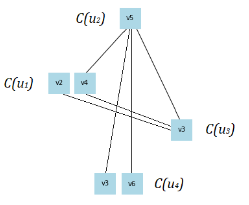
\includegraphics{figures/initcs.png}
        \caption{Initial CS structure}
        \label{fig:dafinitcs}
    \end{figure}

    We use $q' = q^{-1}_D$ for our first refinement. The first vertex will be $u_2$ because it has no children, thus $C'(u_2) = \{v_5\}$
    The second vertex to be processed is $u_1$ because all its children ($u_2$) has been processed already. $v_2$ is not connected with
    any of the candidates of $u_2$. Because of this, $v_2$ will no longer be part of $u_1$'s candidates: $C'(u_1) = \{v_4\}$. The next
    vertex is $u_4$, because its children $u_2$ has been processed. Its new candidates are $C'(u_4) = \{v_3, v_6\}$. The last vertex is
    $u_3$, for which $C'(u_3) = \{v_3\}$. Figure \ref{fig:dafrefcs} shows the CS structure after the first refinement.

    \begin{figure}[h!]
        \centering
        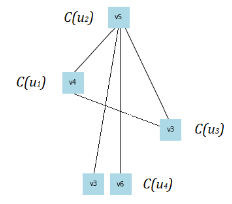
\includegraphics{figures/refinedcs.png}
        \caption{CS structure after the first refinement}
        \label{fig:dafrefcs}
    \end{figure}

    Now $q' = q_D$, however it is not possible to refine CS any further. Next, we find all mappings in CS. The first elements of the 
    search tree is $u_2$ and its candidate ($u_2, v_5$). The set of extendable vertices is $\{u_1, u_4\}$ because their only parent
    $u_2$ in $q_D$ has been processed. We compute the appropriate candidates:

    \[ C_m(u_1) = \{v_4\} \]
    \[ C_m(u_4) = \{v_3, v_6\} \]

    Because of the candidate-size order, we extend the search tree with $u_1$ and its candidate $(u_1, v_4)$. At this point, $u_3$ 
    becomes extendable because its parents were procesed. Its candidates are $C_m(u_3) = \{v_3\}$, and since it is the only extendable
    vertex at the moment, we extend the search tree with $(u_3, v_3)$. The only vertex left is $u_4$. $C_m(u_4) = \{v_3, v_6\}$. The
    search tree is extended with $(u_4, v_3)!$ ($v_3$ is already covered, hence the exclamation mark) and $(u_4, v_6)$. The branch
    containing $(u_4, v_6)$ corresponds to a whole mapping. The failing sets of all nodes on this branch will be empty. The failing set
    of $(u_4, v_3)!$ is $F_m = \{u_3, u_4\}$. In this case, failing sets have no effect on the algorithm. Figure \ref{fig:dafst} shows 
    the search tree with failing sets produced by DAF.

    \begin{figure}[h!]
        \centering
        
        \begin {tikzpicture}[auto, node distance=1cm,thick,main node/.style={circle,draw}]
        \node[main node,label={\scriptsize $F_m = \emptyset$}] (A) {\scriptsize$u_2,v_5$};
        \node[main node,label={\scriptsize $F_m = \emptyset$}] (B) [below=of A] {\scriptsize$u_1,v_4$};
        \node[main node,label={\scriptsize $F_m = \emptyset$}] (C) [below=of B] {\scriptsize$u_3,v_3$};
        \node[main node,label={\scriptsize $F_m = \emptyset$}] (D) [below right =of C] {\scriptsize$u_4,v_6$};    
        \node[main node,red,label={\scriptsize $F_m = \{u_3, u_4\}$}] (E) [below left =of C] {\scriptsize$u_4,v_3!$};    
        \draw (A) -- (B);
        \draw (B) -- (C);
        \draw (C) -- (D);
        \draw (C) -- (E);
        \end{tikzpicture}
        
        \caption{Search tree with failing sets created by DAF}
        \label{fig:dafst}
    \end{figure}

    We got as a result that $q$ is isomorphic to one of $G$'s subgraph and the mapping is the following: $(u_1, v_4),(u_2, v_5),(u_3, v_3),(u_4, v_6)$.

\end{example}
